\documentclass[]{msulabm}
\usepackage[utf8]{inputenc}
\usepackage{amsmath}
\usepackage{graphicx}
%\usepackage[linktocpage]{hyperref}  % if not using colorlinks, use linktocpage
\usepackage[colorlinks]{hyperref}  % if not using colorlinks, use linktocpage
\usepackage{bm}            % bold math
\usepackage{multirow}
\usepackage[table]{xcolor} % provide alternating rows with colors
\usepackage{textcomp}
\usepackage{xfrac} % gives split-level fractions with '\sfrac{a}{b}
\usepackage{multicol}
\usepackage[section]{placeins} % provides \FloatBarrier, to keep floats from crossing this barrier
\usepackage{amssymb}
\usepackage{wrapfig} % provides wrapping figures with text.
%\usepackage{enumitem} % gives \begin{enumerate}[resume] to resume counting from previous enumerate
%\usepackage{subfigure}
%\usepackage{tikz} % to draw arrows
\usepackage{xtab} % provides xtabular, tabular environment that spans multiple pages and other awesome things
\usepackage[style=phys,biblabel=brackets,pageranges=false]{biblatex}
\usepackage{pdflscape}
\usepackage{ragged2e}
\usepackage{longtable}

\bibliography{references-manual,bbarker-zotero}

\newcommand{\abs}[1]{\left\lvert#1\right\rvert}

\title{Laboratory Manual}
\author{PHSC 12700 Stars \\ \\ The University of Chicago}
\date{Autumn 2018}

\pagestyle{ruled}

\definecolor{lgray}{rgb}{.2,.2,.2}

\makeevenfoot{ruled}{\thepage}{\footnotesize{\textit{Last updated \today}}}{}
%\makeevenfoot{ruled}{\thepage}{}}{}
\makeoddfoot{ruled}{}{\color{lgray} \tiny{This work is licensed under \href{http://creativecommons.org/licenses/by-sa/4.0/}{CC BY-SA 4.0} by \href{mailto:bbarker@uchicago.edu}{the University of Chicago}.}}{\thepage}


% allows us to use subcaptions from the memoir class in figures. See Memoir Section 10.9
\newsubfloat{figure}

% don't worry so much about filling every page.
%\raggedbottom

% raise the penalty for splitting footnotes across different pages. Default is 100.
\interfootnotelinepenalty=10000

%\includeonly{amplifier/amplifier} 

% creates a standard length to use 
\newlength{\answerskip}
%\setlength{\answerskip}{90pt} 

%% use plus / minus if latex is squeezing the answer space too much
\setlength{\answerskip}{2cm plus 0.2cm minus 0.2cm}

\newlength{\qaskip}
\setlength{\qaskip}{\answerskip}
\addtolength{\qaskip}{\baselineskip}

% reduce vertical space between chapters in table of contents. Default is 2em.
\setlength{\cftbeforechapterskip}{1em}

% allow for extra line on a page to help prevent widow/orphan lines.
\sloppybottom

% Now we can caption a table outside of the table float environment (good for multi-page tables)
\newfixedcaption{\freetabcaption}{table}

%\includeonly{snells-law/snells-law}
%\includeonly{ohms-law/ohms-law}

\begin{document}
\maxtocdepth{chapter}

 % start roman numbering
 \frontmatter

\maketitle

%\clearpage

%Brent W. Barker

%Department of Astronomy \& Astrophysics

%The University of Chicago

%5640 South Ellis Ave.

%Chicago, IL 60637

%\href{mailto:bbarker@uchicago.edu}{bbarker@uchicago.edu}

%\vspace{2\baselineskip}

%\includegraphics{cc-by-sa-88x31}

%\textcopyright{} 2018 Brent W. Barker. Except where otherwise noted, this work is copyrighted under the Creative Commons Attribution-ShareAlike International 4.0 License. To view a copy of this license, visit \url{http://creativecommons.org/licenses/by-sa/4.0/}.

%\vspace{\baselineskip}

%These labs, excluding "Impulse and Momentum" and the appendices, are a derivative of "\href{https://%sites.google.com/site/scientificabilities/ISLE-labs}{ISLE Labs}" by the Rutgers Physics and Astronomy %Education Research group, used under the Creative Commons Attribution International 4.0 License.
%To view a copy of this license, visit \url{http://creativecommons.org/licenses/by/4.0/}.

%At Rutgers University, many people contributed to this project over the years.
%The list of names is very long and includes: Eugenia Etkina, Alan Van Heuvelen, Suzanne Brahmia, David %Brookes, Michael Gentile, Anna Karelina, Michael Lawrence, Marina Milner-Bolotin, Sahana Murthy, Maria %Ruibal-Villasenor, Aaron Warren, Xueli Zou.

 % skip to next right leaf (``recto'')
 \cleartorecto

 % the star means that the ToC itself is not listed in the ToC
 \tableofcontents*

 % start arabic numbering
\mainmatter 

\chapter{Observing Falling Filters}

	\begin{quotation}
		\textit{The ability to observe without evaluating is the highest form of intelligence.} \sourceatright{Jiddu Krishnamurti}
	\end{quotation}

While Mr.\ Krishnamuri may be making a stretch with his superlative, it remains true that observing without evaluating is essential for the creation of knowledge.
In our lives, we have bias (conceptions, self-constructed mental models) that we use as our lens to view the world.
These models are based on how each of us were socialized and on our subsequent experience.
To learn and create new knowledge, we must develop skill in observation.
In this lab, we will direct you to make detailed, careful quantitative observations, describe the patterns you find with mathematics, and finally make some wild guesses (``hypotheses'') about a more universal principle that explains this pattern that one could use to make predictions.
Due to time and brain constraints, we will not, in this lab, test those hypotheses.

\section*{Learning Goals}

 \begin{itemize}

  \item Conduct an observation experiment, including collecting data, finding and describing a pattern quantitatively, including presentation of data graphically and formulating a quantitative hypothesis.

  \item Use measurement uncertainty to describe physical quantities meaningfully.
  
  \item Format a lab report in a helpful way.
 \end{itemize}

\section*{The Scientific Cycle\protect\footnote{adapted from \cite{etkina_college_2014}}}

Astrophysics is an experimental science. To answer questions, astrophysicists do not just think and dream in their offices but constantly engage in experimental investigations. Astrophysicists use special measuring devices to observe phenomena (natural and planned), describe their observations (carefully record them using words, numbers, graphs, etc.), find repeating features called patterns (for example, the distance traveled by a falling object is directly proportional to the square of the time of flight), and then try to explain these patterns. By doing this, astrophysicists describe and answer the questions of ``why'' or ``how'' the phenomena happened and then deduce quantitative rules called mathematical models that explain the phenomena.

However, a deduced explanation or a mathematical model is not automatically accepted as true. Every model needs to undergo careful testing. When astrophysicists test a model, they use the model to predict the outcomes of new experiments. As long as there is no experiment whose outcome is inconsistent with predictions made using the model, it is not disproved. However, a new experiment could be devised tomorrow whose outcome is not consistent with the prediction made using the model. The point is that there is no way to ``prove'' a model once and for all. At best, the model just hasn't been disproven yet.

A simple example will help you understand some processes that physicists follow when they study the world. One model for the scientific process will also be described (there are other helpful models, and there is no one true ``scientific method''). Imagine that you walk into the house of your acquaintance Bob and see 10 tennis rackets of different quality and sizes. This is an \textbf{observational experiment}. During an observational experiment, a scientist collects data that seem important. Sometimes it is an accidental or unplanned experiment. The scientist has no prior expectation of the outcome. In this case, the number of tennis rackets and their quality and sizes represent the data. Having so many tennis rackets seems unusual to you, so you try to explain the data you collected (or, in other words, to explain why Bob has so many rackets) by devising several hypotheses. A \textbf{hypothesis} is an explanation that usually is based on some mechanism that is behind what is going on, or it can be a mathematical model describing the phenomenon. One hypothesis is that Bob has lots of children and they all play tennis. A second hypothesis is that Bob makes his living by fixing tennis rackets. A third hypothesis is that he is a thief who steals tennis rackets.

How do you decide which hypothesis is correct? You may reason: if Bob has many children who play tennis, and I walk around the house checking the sizes of clothes that I find, then I will find clothes of different sizes. Checking the clothing sizes is a new experiment, called a \textbf{testing experiment}. A testing experiment is different from an observational experiment. In a testing experiment, a specific hypothesis is being ``put on trial.'' This hypothesis is used to construct a clear expectation of the outcome of the experiment. This clear expectation (based on the hypothesis being tested) is called a \textbf{prediction}. So you conduct the testing experiment by walking around the house checking the closets. You do find clothes of different sizes. This is the \textbf{outcome} of your testing experiment. Does it mean for absolute certain that Bob has the rackets because all of his children play tennis? No; he could still be a racket repairman or a thief. Therefore, if the outcome of the testing experiment matches the prediction based on your hypothesis, you cannot say that you proved the hypothesis. All you can say is that you failed to disprove it. However, if you walk around the house and do not find any children's clothes, you can say with more confidence that the number of rackets in the house is not due to Bob having lots of children who play tennis. Still, this conclusion would only be valid if you made an \textbf{assumption}: Bob's children live in the house and wear clothes of different sizes. Generally, in order to reject a hypothesis, you need to check the additional assumptions you made and determine if they are reasonable.

Imagine you have rejected the first hypothesis (you didn't find any children's clothes). Next, you wish to test the hypothesis that Bob is a thief. This is your reasoning: \textit{If} Bob is a thief (the hypothesis), \textit{and} I walk around the house checking every drawer (the testing experiment), \textit{then} I will not find any receipts for the tennis rackets (the prediction). You perform the experiment and you find no receipts. Does it mean that Bob is a thief? He might just be a disorganized father of many children or a busy repairperson. However, if you find all the receipts, you can say with more confidence that he is not a thief (but he could still be a repairperson). Thus it is possible to disprove (rule out) a hypothesis, but it is not possible to prove it once and for all. The process that you went through to create and test your hypothesis is depicted in Figure~\ref{me:fig:isle}. At the end of your investigation you might be left with a hypothesis that you failed to disprove. As an astrophysicist you would now have some confidence in this hypothesis and start using it for practical applications, or \textbf{application experiments}.

\begin{figure}
	\centering
	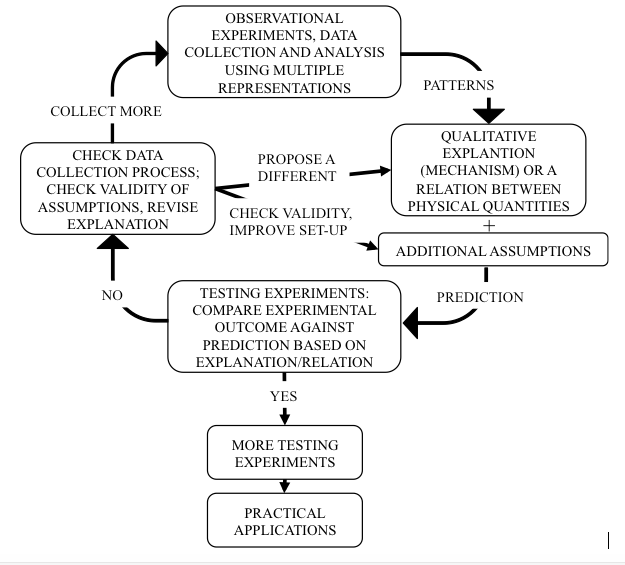
\includegraphics[width=0.7\textwidth]{measurement/islegraphic.png}
	\caption{A model of the process some scientists go through to create knowledge.\cite{etkina_millikan_2015}}\label{me:fig:isle}
\end{figure}

\section*{Observation experiment: Observing falling filters}

In today's lab, you will investigate the relationship between the size of coffee filters and how long it takes them to fall. In the first section, you will determine the size of the coffee filters. In the second, you will determine how long each take to fall, controlling for other variables, and then find a mathematical pattern that describes the relationship. Note that this lab does not include any hypothesis testing.

\begin{framed}
	\textbf{Self-assessment:} To help you improve your scientific abilities, we provide you with self-assessment rubrics.
	A rubric is a scoring system.
	Self-assessment is determining how well you performed a particular task.
	So, these self-assessment rubrics are designed to help you evaluate your performance while you are designing and performing your experiment.
	
	The complete set of rubrics is available in Appendix~\ref{cha:rubrics}.
	In each lab, your report will be assessed using Rubric F, found in Table~\ref{rubric:f}, as well as 5 additional rubric rows listed in that lab.
	Each week, read through these and use them to evaluate your work as you design and perform the experiment.
	Your instructor will use the same rubrics to determine part of your grade for the lab.
	We will use the other rubrics in future labs.
\end{framed}	

\textbf{Rubrics to focus on during this experiment:} B5, B7, B8, F1, F2, G1, G2. See Appendix~\ref{cha:rubrics} for details.

\textbf{Available equipment:} several differently-sized coffee filters, meter stick, balance or scale, stopwatch, scratch paper%, camera (on your phone), Computer with ImageJ installed, string

\subsection{How big are the filters?}

% DevNote: I decided to not make this a whole application experiment with 2 different methods, for the sake of time. I also removed image analysis with ImageJ, for the same reason. --bbarker, 2018-10-02

\textbf{Goal:} Find the cross-sectional area of each coffee filter and make a determination of that area, including uncertainty in that area, for use in the next section.
%In Stage 1 of the Barker X-Prize, each team has been tasked with determining precisely how big various objects are, including marbles, cotton balls, and coffee filters, including a detailed determination of their uncertainty of these measurements.
 
%\begin{framed}
%	ImageJ is an image analysis program that includes, among other things, the ability to measure lengths, angles, and areas in images, provided that you give it a scale for how long some reference object is in the image.
%\end{framed}

\begin{enumerate}
	\item You may want to \textbf{decide on roles} for each group member. Example roles include Facilitator (ensures time and group focus are efficiently used), Scribe (ensures work is recorded), Technician (oversees apparatus assembly, usage), Skeptic (ensures group is questioning itself). Note that each role is responsible for ensuring that the thing happens, rather than necessarily doing it themselves. 
	
	\item Review Rubric G (Table~\ref{rubric:g}) and discuss any unclear expectations with your group and the instructor.
	
	\item Discuss with your group what cross-sectional area means and why it might affect the fall time. Feel free to use your resources (books, internet, etc.) to do this.
	
	\item Brainstorm different methods you could use to determine the cross-sectional area. Feel free to play with the equipment as desired. Here are some things to consider:
	\begin{itemize}
		\item Will you measure the area directly, or will you measure something else and use that to calculate the area?
		
		\item With any method, you will probably make one or more assumptions about the shape of the filter. How valid are those assumptions?
		
		\item For each method you consider, there may be different sources of uncertainty --- the resolution of the measuring devices themselves, how you use them to measure, etc. If there is a source of random uncertainty, then you will need to take several measurements and use Appendix~\ref{unc:random} to determine the uncertainty. The decision of how many measurements to take is a trade-off between increasing precision (decreasing the uncertainty of the mean) and decreasing the time the measurement process takes.
		
		\item If you make a measurement and use that measurement in an equation to find the area, you will need to propagate uncertainty as described in Appendix~\ref{unc:sec:prop}.
	\end{itemize}
	% Come up with two independent methods for determining the cross-sectional area. The purpose is that if you make a mistake or wrong assumption in one method, then the method (hopefully) gives a different result than the other method. For discovering new things, this is one quantitative way of checking your work, since you don't have the answer ahead of time.
	
	
	
	\item Decide on your method and discuss it with an instructor before you begin. They will help increase the chances that your method will lead to successful results, or at least that the unhelpful path that you choose will take a short enough amount of time for you to change it when you discover it does not work. We want you to have productive failure that you have time to learn from.
	
	\item Write down an outline of your intended procedure. You might end up changing this as you go, but it is helpful to start with a plan and then change it, rather than having no plan at all.
	
	\item For your procedure, list the sources of uncertainty involved with each measurement. For each source, identify whether it is a random or instrumental uncertainty.
	
	\item Execute your procedure, including setup, data collection, calculation of area, uncertainty estimation and propagation.
	
	\begin{framed}
	At the end of this step, you should have a table of coffee filter cross-sectional areas, with uncertainties.
	\end{framed}
	
	\item Once you are done collecting this data, review your written procedure and correct it to match what you actually did, and ensure you have sketched any measurement setups, so you can include it in the lab report. In particular, ensure that you have enough written so you can demonstrate Rubric Rows F1, G1 and G2 in your report (see Tables~\ref{rubric:f} and \ref{rubric:g}).
	
\end{enumerate}
 
\subsection{How fast do the filters fall?}

\textbf{Goal:} Determine how long it takes each coffee filter to fall.

\begin{enumerate}
	\item Review Rubric B (Table~\ref{rubric:b}) and discuss any unclear expectations with your group and the instructor.
	
	\item Identify any variables (things that could change between measurements --- either between measurements of the same filter, or among different filters) that could affect the fall time other than the coffee filter's cross-sectional area. If there is controversy in the group, feel free to test what variables might affect that fall time.
	
	\item Since you are testing how the fall time is related to the filter's area, you should hold the other variables constant, so that they affect all the filters in the same way. For each variable identified in the previous step, decide how to keep that constant.
	
	\item Brainstorm different methods you could use to determine the time it takes for the filter to fall. Feel free to play with the equipment as desired. Here are some things to consider:
	\begin{itemize}
		
		\item Will you measure the fall time directly, or will you measure something else and use that to calculate the area?
		
		\item For each method you consider, there may be different sources of uncertainty --- the resolution of the measuring devices themselves, how you use them to measure, etc. If there is a source of random uncertainty, then you will need to take several measurements and use Appendix~\ref{unc:random} to determine the uncertainty.
		
		\item If you make a measurement and use that measurement in an equation to find the time, you will need to propagate uncertainty as described in Appendix~\ref{unc:sec:prop}.
	\end{itemize}
		
	\item Decide on your method and discuss it with an instructor before you begin. They will help increase the chances that your method will lead to successful results, or at least that the unhelpful path that you choose will take a short enough amount of time for you to change it when you discover it does not work. We want you to have productive failure that you have time to learn from.
	
	\item Write down an outline of your intended procedure. You might end up changing this as you go, but it is helpful to start with a plan and then change it, rather than having no plan at all.
	
	\item For your procedure, list the sources of uncertainty involved with each measurement. For each source, identify whether it is a random or instrumental uncertainty.
	
	\item Execute your procedure, including setup, data collection, calculation of area, uncertainty estimation and propagation.
	
	\begin{framed}
	At the end of this step, you should have a table of coffee filter cross-sectional areas, with uncertainties, with another column for fall time, with uncertainty in the fall time.
	\end{framed}
	
	\item Once you are done collecting this data, review your written procedure and correct it to match what you actually did, and ensure you have sketched any measurement setups, so you can include it in the lab report. In particular, ensure that you have enough written so you can demonstrate Rubric Rows B5, F1, G1 and G2 in your report (see Tables~\ref{rubric:b}, \ref{rubric:f}, and \ref{rubric:g}).
\end{enumerate}

Now that you have these measurements, it is time to find a pattern.

\subsection{Finding a pattern}

The penultimate step in an observational experiment is to find a pattern. Note that we are not explaining why this pattern is happening yet --- we are focusing on describing it first.

\textbf{Goal:} Find a pattern in the data and describe it mathematically.
\textbf{Available equipment:} Computer with spreadsheet software

\begin{enumerate}
	\item Use a plotting program, for example LibreOffice Calc or Microsoft Excel, to plot a graph of fall time vs. filter area. The independent variable should be on the horizontal axis. The axes should each be labeled with the quantity name and the unit in parentheses. For example, if you measured fall time in seconds, then the axis label should be something like ``fall time (s)''.
	
	\item In that graph, include also the uncertainty in each value. This usually involves right-clicking on a data point and selecting ``error bars''. Then you can highlight the column of cells that include the uncertainties.
	
	\item Visually, discuss what shape the data points make. Speculate what kind of relationship you see. Is it proportional? Linear? Parabolic? Exponential? Logarithmic?
	
	\item Create a line of best fit (or ``trend line'') in the graph using the software. Choose the equation type to match what your group guessed in the previous step. If the line obviously does not match the data, try again with a different equation type. Quantitatively, the goodness of fit of a line (how close the line is to your data points) can be represented by the correlation coefficient, given as $r^2$ in the software. If $r^2 \gtrsim 0.8$, then the equation that you found describes the data fairly well.
	
	\item Review Rubric Rows B7 and B8 in Table~\ref{rubric:b} and ensure that you are demonstrating them here or have enough information to do so in your lab report.
\end{enumerate}

\subsection{Finishing up}

XXXX TO FINISH XXXX

what to include in lab report

extra fun: extrapolate to 0 area, compare with freefall time.

%Rationale:
%\begin{enumerate}
% \item want one experiment where students measure lengths and estimate uncertainties that are needed for data analysis. Lengths are intuitive things for students, no prior teaching needed. Then they see how those lengths compare to something else in a physics-y way. Then they graph it and decide what functions might describe them.
 
% \item falling and air resistance is good here. air resistance depends on cross sectional area, so length measurement. Data is not simple and obvious, but is instead messy, making pattern identification non-trivial, but still possible. Also cannot just use or look-up simple answers online -> authentic inquiry.
 
% \item so could do area vs. time to hit the floor. Can measure with video tracking, photogates, motion detector, stopwatch. need multiple sizes of coffee filters.
 
% \item Or position vs. time for different objects. This should give some interesting graphs, since objects can vary from no-meaningful-air-resistance to dominated-by-air-resistance constant. And the latter case should have an acceleration at the beginning, then constant, so it's more complicated. Must use video tracking or motion detection. So includes the skill of choosing with data to model. is there one function that works for all parts, or is there a transition between different situations?
 
% \item for video tracking, need to know how students can find framerate of videos they take, make sure it's easily imported to OSP Tracker.
%\end{enumerate}

\section{If in Stars class, also do this:}
\subsection{Remote Observing with the Stone Edge Observatory}

For two labs in this course, we will be taking observations remotely with the Stone Edge Observatory in Sonoma, California. We will use a queuing system to submit observations that are automatically scheduled and taken by the telescope. The data are then processed and typically available for analysis several days after they were obtained. To ensure that our data are taken and reduced in time for our in-lab analysis (which is subject to possible delays due to, e.g., the weather at the observing site), we will be submitting observations to the queue several weeks prior to lab in which they will be analyzed.

First, you will need to register for an account that will allow you to access the queue website. Make groups of two to three students so that there are no more than 5 groups in a section. Each group will use one member’s email to sign up for an account in the queuing system. A TA will be present to manually add each group. Each group will receive an email that will allow them to create an account. Since you will be sharing an account, be sure to share the account password (and obviously don't re-use one from another personal account).

Once you have an account, you will be able to log onto the queue and submit observations. To do so, go to the website \texttt{https://queue.stoneedgeobservatory.com/} and log-in with your group's credentials. Then navigate to \texttt{OBSERVATIONS} $\blacktriangleright$ \texttt{SUBMIT AN OBSERVATION}. This will take you to a form that allows you to input the specifics of your observation. These will be given to you for each lab.

\subsection{HR Diagram: Taking observations}
For this lab, each section will be taking observations of one of two star clusters --- NGC 869 and M15. You will then use this data to make color-magnitude diagrams of these clusters, which can then be compared with stellar evolution models to determine when these clusters formed. Table~\ref{hr_diagram_obs} lists the parameters for the observations to be taken in this lab - each section will be assigned a cluster, and each group in the section should submit one observation. Each group will then analyze their data in-lab, and will combine datasets. If there are fewer groups than observations, omit the longest-exposure observations.

\begin{table}
    \centering
    \caption{HR Diagram Lab Observations}
    \label{hr_diagram_obs}
    \begin{tabular}{|l|c|c|c|c|r|}
    \hline
    \textbf{Program} & \textbf{Target} & \textbf{Exp Time (s)} & \textbf{Exp Count} & \textbf{Bin}
         & \textbf{Filters} \\
    \hline
    General & M 15 & 1 & 1 & 2 & Dark, g', r'\\
    \hline
    '' & '' & 5 & '' & '' & '' \\
    \hline
    '' & '' & 10 & '' & '' & '' \\
    \hline
    '' & '' & 20 & '' & '' & '' \\
    \hline
    '' & '' & 40 & '' & '' & '' \\
    \hline
    '' & NGC 869 & 0.5 & '' & '' & ''\\
    \hline
    '' & '' & 1 & '' & '' & '' \\
    \hline
    '' & '' & 2 & '' & '' & '' \\
    \hline
    '' & '' & 5 & '' & '' & '' \\
    \hline
    '' & '' & 10 & '' & '' & '' \\
    \hline
    \end{tabular}
\end{table}

\section{Post-lab survey}

[Include Anna Karelina's flow questions here]

\chapter{Spectroscopy}

\section{Introduction}

In this lab we will study light produced in gas discharge tubes.
You will first familiarize yourself with operation of the software by making careful measurements of emission lines from a hydrogen discharge tube.
You will then use your knowledge of spectra to identify which elements are present in several other discharge tubes.

\section{Learning goals}

\begin{itemize}
	\item Use experimentally derived quantities to calculate the Rydberg constant.
	\item Identify unknown elements based on their spectra.
	\item Compare continuum vs.\ line emission.
	\item Demonstrate an ability to make careful measurements.
	\item Demonstrate proficiency in basic calculations and plotting using spreadsheets.
	\item Gain familiarity with a common physics tool (the spectroscope).
\end{itemize}

\section{Scientific background}

When an electron collides with an atom in the discharge tube, the atom absorbs energy and transitions from its \textit{ground state} to an \textit{excited state}.
When the atom later transitions back to its ground state, it emits energy in the form of light.
Light from these transitions is emitted only at distinct colors, or wavelengths.
The wavelengths of the spectral lines from each element are different, thus each element has it own ``fingerprint'' by which it can be identified.
Spectroscopy can therefore be used to detect and measure elements in a material from a distance.
Critically, the same lines that appear in gas discharge tubes the lab are also found in stars, allowing astronomers to study their elemental makeup.
Without spectral information, there would be no other way for us to know what stars are made of because we cannot travel and take a sample, even for the closest star --- our Sun.

As with much of astrophysics, we'll begin by studying the properties of hydrogen.
Although hydrogen is the most abundant element in the universe, its lines in the sun are
quite weak because the strength of the lines depends critically on the physical conditions
in the star. Hydrogen was first identified on earth by Anders Jonas Ångström in 1853, but
it was not detected in the sun until a decade later. Although Ångström was able to
measure the four characteristic lines of hydrogen --- known today as H$\alpha$, H$\beta$, H$\gamma$, and H$\delta$ --- to a high degree of accuracy, it was not until 1885 that Johann Balmer (a sixty year old
Swiss school teacher and mathematician with no physics background) found the correct
mathematical relationship between the wavelengths of hydrogen. Balmer's relation suggested that the physical processes which produce hydrogen lines are connected to
integer numbers, an explanation that ultimately required the overthrow of 19th century
classical physics in favor of the first version of quantum theory by Bohr and others circa
1915.

The four Balmer lines correspond to transitions to the $n=2$ state in hydrogen %TODO (see Figure~???)
and follow the equation
\begin{equation}\label{spec:eqn:balmer}
 \frac{1}{\lambda} = R \left( \frac{1}{n^2_\textrm{final}} - \frac{1}{n^2_\textrm{initial}} \right)
 = R \left( \frac{1}{4} - \frac{1}{n^2_\textrm{initial}} \right) \,,
\end{equation}
where $\lambda$ is the wavelength of a particular line and $R = 1.097 \times 10^7\:\mathrm{m}^{-1}$ is the Rydberg constant, with $n_\textrm{initial}>2$.

\section{Apparatus description: spectrometer}

To measure spectral lines, astronomers use a device called a spectrometer, spectroscope, or spectrograph. Spectrometers used for precision scientific measurements have three basic elements:
\begin{enumerate}
	\item A collimator consisting of a slit and mirror or lens. The collimator produces a
parallel beam of light in one direction, similar to an eyepiece of a telescope

	\item A dispersive grating that bends the light at an angle that depends on the
wavelength of light, thereby decomposing it into a spectrum

	\item A mirror or lens that collects the light and focuses it onto a detector
The main part of any spectrograph is a dispersive element, which is usually a grating that
consists of a very finely spaced lines etched on a substrate. The spacing between the
lines can be 1/10 of the diameter of a human hair and the distance between each line is
controlled to less than the diameter of a single atom. The process used to etch the grating
is similar to that used in making CDs. Not surprisingly, CDs can be used to decompose a
white light from a lamp into rainbow.%TODO, as shown in Figure ???.
\end{enumerate}

The angle $\theta$ at which grating reflects the light depends on the wavelength and is given by
\begin{equation}
 m \lambda = d \sin{\theta}\,,
\end{equation}
where $m$ is the order of the maximum, $\lambda$ is the wavelength (generally measured in nanometers, where a nanometer is $10^{-9}$ meters), $d$ is the spacing of the lines on the diffraction grating (also in nm). Visible light has a wavelength of about $500\:$nm.

\section{Apparatus: the digital spectrometer}

A digital spectrometer also uses a diffraction grating, but instead of collecting the dispersed light on a screen to be viewed by people, it collects the light with a charge-coupled device (CCD), an array of light-sensitive pixels much like a digital camera. It then translates the position on the CCD to individual wavelengths and displays a plot of intensity vs. wavelength on a computer. %TODO (see Figure~???)
Another difference is that we use an optical fiber to collect the light.

Here are a few guidelines:
\begin{itemize}
	\item Save the images of spectra and numeric files that you generated with SpectraSuite
	during your experiments on a USB stick, so that you can use them at home during
	preparation of your report (you can also email them as attachments from your
	computer at the end of the lab).
	
	\item You should open a word processor document and a spreadsheet document in which you can save your measured
	spectra at the beginning of your work. To save an image of your graph, click on
	the fourth icon from the left in the Spectrum IO controls. %TODO (Fig.~???)
	This will copy
	an image of the graph to the clipboard. Then in your word processor, paste the image by pressing
	Ctrl-V.
	
	\item To save spectrum in the digital form, click on the third from the left icon in
	Spectrum IO controls (to the right of print icon). This copies it to clipboard. In
	Excel file make sure you are in a new sheet and press Ctrl-V. This should create
	to columns of numbers: wavelength (in nm) and counts for your spectrum.
	
	\item An alternative way to save the data is to click on the floppy disk icon in the
	Spectrum IO controls. The format must be ``Tab delimiter, no header''. The
	writing directory must be specified (``Browse'' button). The spectrum is saved in a
	text file (.txt) as two columns, the first column giving the wavelength in nm, the
	second column the corresponding intensity. This file can be imported into a spreadsheet or plotting program.
\end{itemize}

\section{Observation experiment: Spectrum of the sky and of fluorescent lamps}

\textbf{Goal:} Observe the spectrum of the sky and of the fluorescent lights in the room, notice the differences, and identify some elements present in the fluorescent light bulb.

\textbf{Rubric rows to focus on:} B5, F1, F2.  See Appendix~\ref{cha:rubrics} for details.

\textbf{Available equipment:} Ocean Optics Red Tide digital spectrometer with USB cable and fiber optic cable attached, computer with SpectraSuite software, window with daylight visible (or incandescent bulb if night-time lab), fluorescent light source

\begin{framed}
	\textbf{Caution: Fragile Equipment!} The fiber optic cable is a precision instrument. If it is bent in too tight a curve, it will be damaged. Do not bend these cables beyond a $12\:$cm radius ($4.5\:$inches) (into part of a circle with a radius smaller than that).
	
	Also, the openings have covers to protect from dust and debris. Be sure to replace the end cover when you are done with the cable.
\end{framed}

\begin{enumerate}
	\item Turn on the computer and start Spectra Suite.
	
	\item Ensure the digital spectrometer is connected to the computer and the fiber optic cable is connected to the spectrometer.
	
	\item Remove the blue end cap from the fiber optic cable by twisting it.
	
	\item Press S (``Scope'') to start measuring the spectrum %TODO (see Figure~???)
	and point the fiber towards the overhead fluorescent light. You should see live spectrum of the light
	entering the fiber in the graph window, which is characterized by many strong peaks
	(strong emission lines).
	
\begin{framed}
	A \textbf{fluorescent lamp tube} is filled with a gas containing low pressure mercury vapor,
		argon, neon, xenon or krypton, with corresponding lines in the spectrum. Emission lines
		are also produced by a phosphorous material (typically europium and terbium) covering
		the glass, after excitation by the ultraviolet emission from the lamp gas.
\end{framed}

	\item Record a spectrum and identify the different lines and their corresponding element, by
	comparison with other measurements of fluorescent light spectra (see Table~\ref{spec:tab:emissions}). Save the spectrum and
	include it in your lab report along with markers of lines that you were able to identify.
	
	\item Once you examine the spectrum you obtained with spectrometer, look at it with the visual
	spectroscope and identify lines you see visually with the lines you see in the digital
	spectrum.
	
	\item Repeat the above procedure, but looking out a window at the sky. Record what you see,
	and make notes of how the spectrum from the sky differs from the spectrum of the
	fluorescent lights.

\end{enumerate}

\section{Application experiment: Measuring the Rydberg constant}\label{spec:sec:rydberg}

\textbf{Goal:} Measure the wavelengths of light emitted from electrified hydrogen gas, and use those wavelengths to determine the Rydberg constant.

\textbf{Rubrics rows to focus on:} D4, D7, F1, F2, G2, G4. See Appendix~\ref{cha:rubrics} for details.

\textbf{Available equipment:} direct viewing spectrometer, Ocean Optics Red Tide digital spectrometer with USB cable and fiber optic cable attached, computer with SpectraSuite software, gas discharge tube power supply, hydrogen gas discharge tube

\begin{framed}
 \textbf{Warning: Shock Hazard!} When turned on, the power supply generates $5000\:$V of electric potential difference across the terminals, with enough current available to injure you. Make sure that the discharge tube has its ON/OFF switch (on the side) in the
 OFF position when you install or change the discharge tube. If not, switch the lamp into
 the OFF position. Switch on the lamp to ON position only after tube is installed. The
 lamp will now be illuminated when the pedal is pressed. While the pedal is pressed, do not touch any part of the tube. Moving the
 whole unit by the base is safe.
\end{framed}

\begin{framed}
	\textbf{Caution: Fragile Tube!} Avoid touching the tube with your skin, as skin oils can degrade the glass over time. Wear a nitrile glove when touching a tube.
	
	Also, the tubes have a limited lifetime of running. Turn on the tube only for as long as you need it to be on for measurement.
\end{framed}

\begin{enumerate}
	\item Ensure that the hydrogen tube is installed in the power supply.
	
	\item Turn on the power supply and examine its spectrum through a direct viewing spectroscope. You should be able to see a bright
	magenta and a cyan line --- these are the first two lines in the Balmer series. The other two
	lines are probably too faint for you to see; in order to measure them, we will need to use a
	more sensitive device.
	
	\item Observe using the digital spectrometer by starting the SpectraSuite software, uncapping the optical fiber, and placing it as close as possible to the discharge tube and turn on the lamp. Adjust
	pointing of the fiber so that the height of the lines in the acquired spectrum is maximized.
	If the strongest lines are saturated, you can either move the fiber a bit farther away from
	the discharge tube or adjust integration time within the SpectraSuite software.
	
	\item Follow these steps to measure the spectrum of light that enters the fiber using controls of the SpectraSuite software: %TODO (Figure~???):
	\begin{enumerate}
		\item Make sure you are in a new graph and enter Scope mode by pressing S in the
		controls. Point fiber at the discharge tube.
		
		\item Take a background ``dark'' measurement with the light source under study off by
		clicking the gray light bulb button in spectrum storage controls%TODO (Figure~???)
		
		\item Subtract the background spectrum from the signal by clicking gray light bulb with
		minus sign button in the Processing controls. This removes contribution of
		background light to the spectrum.
		
		\item turn on the source discharge tube and record its spectrum, saving an image of it as describe above in the guidelines.
		
		\item While source is on, click on the spectrum graph. You should see a peak icon in the
		bottom right corner of the graph. This is useful peak finder: click on it and adjust
		controls, setting the Baseline, which is the intensity above which it will search for peaks. Peak finder identifies peaks and you can step through them and see their
		wavelengths using $<$ and $>$ buttons in the bottom left corner of the graph.
	\end{enumerate}

	\item You should adjust the setup and acquisition time so that you can easily see four peaks
	(emission lines in the spectrum). Analyze the spectra and determine the wavelength of
	the four most prominent lines. Assume that these wavelength measurements are exact for the purposes of uncertainty analysis.
	
	\item\label{spec:step:rydberg} Write down the measured wavelengths of each line in the descending order of
	wavelength ($n_1 =3$ corresponds to the peak with the longest wavelength that you measure,
	while $n_1 = 6$ to the shortest of the four you measure) in a table like Table~\ref{spec:tab:rydberg}. Be careful to
	measure the correct lines! The spectrometer is sensitive to wavelength is the near infrared
	and near ultraviolet, beyond detection of the human eye. Do you observe any such lines?
	Can they be included in your analysis?
\end{enumerate}

\begin{table}
	\centering
	\begin{tabular}{c|c|c}
		\textbf{Energy level ($n$)} & \textbf{Measured Wavelength (nm)} & \textbf{Rydberg constant (nm$^{-1}$)} \\ \midrule
		3 & & \\ \midrule
		4 & & \\ \midrule
		5 & & \\ \midrule
		6 & & \\ \bottomrule
	\end{tabular}
	\caption{Suggested table for recording data for Step~\ref{spec:step:rydberg} in Section~\ref{spec:sec:rydberg}.}\label{spec:tab:rydberg}
\end{table}

\subsection{Analysis}

Using your data for each line, calculate the corresponding value of the
Rydberg constant in units of 1/nm using Equation~\ref{spec:eqn:balmer} and enter it into the column for the Rydberg constant
in each line's row. The spectral lines you observe correspond to the first four transitions
in the Balmer series, the transitions of electrons to the $n_\mathrm{final}=2$ level from higher energy
levels.

The differences in values you get for the Rydberg constant are due to random uncertainty. To find your determination for this quantity, use your average for the value, and calculate the standard deviation for the uncertainty.

A more sophisticated way of calculating the Rydberg constant would be to plot a graph of
your measurements of $1/\lambda$ vs $1/n_i^2$ and fit a straight line through it. The
average value of the Rydberg constant is the slope of this line, which will be given by the
slope. Carry out and present such a measurement along with the plot in your report.

\section{Application experiment: identification of mystery elements}

\textbf{Goal:} Identify the gas that is contained in the four tubes with colored tape on them.

\textbf{Rubric rows to focus on:} F1, F2

\textbf{Available equipment:} Ocean Optics Red Tide digital spectrometer with USB cable and fiber optic cable attached, computer with SpectraSuite software, gas discharge tube power supply, various gas discharge tubes with unknown gases

Turn off the lamp using the switch on the side, and replace glass tube with hydrogen gas
with one of the color-coded bulbs that will be provided to you. As before, use the
spectrometer to acquire spectrum using the SpectraSuite software and measure
wavelengths of the prominent lines (peaks in the spectrum).

Once you have measured a few prominent wavelengths, compare them with wavelengths
of known lines of elements listed in the table below and identify the mystery element
within the color-coded tube. Present your measurements of wavelengths in a list and a
plot of the graph with several lines from Table~\ref{spec:tab:emissions}.

\begin{table}
	\centering
	\begin{tabular}{c|c|c|c}
		\toprule
		\textbf{Helium (nm)} & \textbf{Argon (nm)} & \textbf{Neon (nm)} & \textbf{Mercury (nm)} \\ \midrule
		389 & 697 & 585 & 365 \\
		447 & 707 & 594 & 404 \\
		469 & 738 & 614 & 435 \\
		492 & 751 & 627 & 546 \\
		502 & 764 & 640 & 579 \\
		588 & 772 & 651 & \\
		668 & 795 & 660 & \\
		707 & 801 & 668 & \\
		727 & 811 & 693 & \\
		& 826 & 703 & \\
		& 841 & 717 & \\
		& 852 & 744 & \\
		& 866 & & \\
		& 912 & & \\ \bottomrule
	\end{tabular}
	\caption{Some known emission lines of various elements.}\label{spec:tab:emissions}
\end{table}

\section{End of Lab - Queue observations for 61 Cygnus AB}

As we did in the first lab session, we will end this lab by queuing observations for a future lab. Specifically, each group will take an observation of the binary star system 61 Cygnus AB. The observational parameters are listed in Table~\ref{61Cyg_obs}. Refer to the previous chapter for instructions on submitting observations.

\begin{table}
	\centering
	\caption{61 Cyg AB Observations}
	\label{61Cyg_obs}
	\begin{tabular}{|l|c|c|c|c|r|}
		\hline
		\textbf{Program} & \textbf{Target} & \textbf{Exp Time (s)} & \textbf{Exp Count} & \textbf{Bin}
		& \textbf{Filters} \\
		\hline
		General & 61 Cyg & 1 & 1 & 2 & Dark, g' \\
		\hline
	\end{tabular}
\end{table}
\chapter{The HR-Diagram}

\section{Introduction}

In this lab we will analyze our observations of star clusters to make one of the key figures in all of observational astronomy - the Hertzsprung-Russell (HR) Diagram. This will give us insight into the stellar populations in the clusters we observe, and allow for an estimate of the cluster ages. 

\section{Learning goals}

\begin{itemize}
    \item Gain an understanding of astronomical image analysis and photometry
	\item Gain practice performing basic calculations on datasets and making informative scientific figures from those data
	\item Learn where different stellar populations lie on the HR diagram, and understand the physical reasons behind these localizations
	\item Estimate stellar cluster ages using the predictions of stellar evolutionary models. 
\end{itemize}

\section{Scientific background}

Stars evolve (i.e., change their properties) over millions and often billions of years – too slow for us to see the evolution over a human lifespan.  Such impressive longevity is due to the fact that stars are powered by thermonuclear reactions, which are very efficient in generating abundant energy and have quite a bit of fuel to last for a long time. Stars like our Sun last about 10 billion years (so the Sun is in its middle age). The long timescale of evolution also means that we have to develop a different way to study stellar evolution. 

Astronomers explore evolution of stars by observing large populations of stars where different stars are in different stages of evolution. Of course, in order to do this we need to be able to tell which star is in what stage. This is done by a combination of observations – which measure luminosity and surface temperatures – and theoretical models – which predict how luminosity and surface temperature change as stars evolve. The key is that luminosity and temperature at a certain age are determined by star's mass, chemical composition, and details of thermonuclear reactions (which elements are burning, over what fraction of star's volume, etc.).

Luminosity and temperature of stars are related because they are both determined by their internal structure, which, in turn, is determined by the basic physical properties (mass, chemical composition, age). Therefore, stars are not scattered randomly in the luminosity and temperature space but follow well-defined sequences, which reflect the ranges of the controlling parameters in a given stellar population. 

The surface temperatures of stars can be deduced by fitting a blackbody radiation spectrum to their spectra. Even for stars that do not have spectra measured, their temperatures can be deduced from their colors (Recall: does bluer color correspond to cooler or hotter temperature?). Our eyes and brain perceive color by analyzing spectral composition of the incoming light. In astronomy, a star's color is defined as the difference between its magnitudes measured through two different filters that block out all light except light within a fairly narrow range of wavelengths. 

In order to interpret evolutionary states, we look at physical groupings of stars called stellar clusters, which are located at the same distance from us and were born at the same time from the same cloud of dense gas. The spread in their properties will thus not be due to different ages or initial compositions, but mainly due to different masses. As you will see, stars occupy distinct regions of the observable equivalent of the luminosity-temperature space – the magnitude-color space called the Hertzsprung-Russell (HR) diagram. We will make this diagram for the star cluster we observed.

\section{Obtaining Images}

To view images taken by the SEO and download the associated data, sign into your account on the queue website (\texttt{https://queue.stoneedgeobservatory.com/}), navigate to \texttt{OBSERVATIONS} $\blacktriangleright$ \texttt{MY OBSERVATIONS}. The observation you queued should be listed, and \texttt{Yes} should appear in the \texttt{Completed} column if the data have been taken. To view and download completed observations, click \texttt{Actions} $\blacktriangleright$ \texttt{Go To Images}. This will link you to an external page with both an image viewer and links(?) to directly download the data. This can be accomplished with the \texttt{Download Selected FITS File}. Make sure that the \texttt{Pipe Step} option under \texttt{Selection} is listed as \texttt{FludxCalibrated}, since this is the reduced and calibrated data. There are other data products from both the observation and data reduction process available from this page, but we aren't using them for our analysis. Unfortunately, the data reduction process does not work on every observation, so if one or both of your observations lacks \texttt{FluxCalibrated} option, share data with a group that does.\textit{Note that you cannot use data from different observations for both filters - i.e. observations from both filters analyzed by each group need to be of the same exposure time}. Download these data onto your local machine where you will perform your analysis.

\section{Analyzing the data in DS9}

To analyze our observations we will be using DS9 (\texttt{http://ds9.si.edu/site/Home.html}), a popular software package for the visualization and basic analysis of image data within the astronomical community. If you are working on a lab computer, the software is already installed. If you are using your personal computer, it can be downloaded and installed from the provided link. 

We will use this tool to measure the flux in both observed filters for as many stars as possible. Each group should use separate, adjacent computers - bring up images in DS9 for each filter, one filter per computer. To better visualize the images in DS9, logarithmically scale the display by selecting \texttt{scale} $\blacktriangleright$ \texttt{log}. Contrast and bias of the display image can be modified by clicking and dragging - you should adjust these so that the stars are optimally visible.

To determine how much flux comes form each star, we will use the ``regions" functionality of DS9 that gives information about a selected region in the image. First click \texttt{edit} $\blacktriangleright$ \texttt{region}, and then you will create a region -- indicated by a green circle -- each time you click on the image. Clicking in the center of the region will allow you to move it about the image, while clicking on the edge allows you to adjust it's size. For each star you measure, you'll want to create a region that contains as much flux as possible without contamination from a nearby star or the background. Once this is accomplished, double click the region (which will cause a window with basic information to appear), and select \texttt{Analysis} $\blacktriangleright$ \texttt{Statistics}, which will cause a separate panel to appear with information about the data contained in that region. ``Sum" is the flux (in an astronomy-specific unit called ``Janskys", abbreviated as Jy) value you should record. Also recod the ``Center" coordinates and radius of the region. Do this in both filters, for each star that you measure. \textit{Note that the error listed under ``Statistics" is \textbf{not} a correct estimate of the error in the flux value, so do not record this}.

Error in your measurement can be the result of several causes, but one that is easy to quantify is the presence of background noise (from e.g. sky brightness or scattered light in the telescope). From several circular regions over nothing in particular, determine how many counts there are per unit area, just from the backgrounds.  The “surf$\_$bri” value gives what we need.  Do this several times to determine the variance in the background, and also how it varies over the different parts of the image.  Thus quantify this background and its error. For each of your stars, compute the background that was likely in the aperture.  This involves multiplying the surface brightness by the area you chose.  The error in the surface brightness propagates, so if you have a very big region, that will likely determine the error on your final measurement. 

Try to measure fluxes and errors for as many stars as possible in your lab session. There will inevitably be some overlap between groups, which is fine, but try to obtain measurements for stars at a wide range of brightness’s. 50 stars is a good target, but the more the better. Thirty minutes before lab ends, stop collecting data, and share your data among your section so that you can finish the rest of the analysis.

\section{Calculating Magnitudes}

In astronomy we deal with magnitudes, which are scaled logarithmically, and increase with decreasing source brightness. Specifically, the equation for the magnitude $m_X$ of an object in a wavelength band $X$ with flux $F_X$ is given by 

\begin{equation}
m_{X} = -2.5\log_{10}\left(\frac{F_X}{F_{X,{\textrm{ref}}}}\right)
\end{equation}

where $F_{X,{\textrm{ref}}}$ is a reference flux value for the given band and magnitude system. For the SDSS magnitude system we are using, $F_{\textrm{ref}} = 3631 {\textrm{Jy}}$ for both $g'$ and $r'$ measurements. Calculate magnitudes in both bands for all of the stars measured in your section. You can use Excel or any other software/coding language of your choice to do this.  

\section{Making an HR Diagram}

Since different bands measure brightness in different wavelengths, the ratio of flux in two bands is a measure of an object's color. Therefore, the difference between astronomical magnitudes of an object in different bands is a measure of its color, since the magnitude scale is logarithmic:

\begin{equation}
m_A - m_B = -2.5\log\left(\frac{F_A}{F_B}\right).
\end{equation}

An H-R diagram is a plot of stellar magnitude vs. color - aka a ``color magnitude diagram''. A star's color is an observational indication of it's surface temperature. Since all of the stars in a star cluster are at approximately the same distance, their apparent magnitude gives a good relative indicator of luminosity. Therefore, a color-magnitude diagram of stars at roughly constant distance is effectively a temperature-luminosity diagram, and stars fall in characteristic regions of this parameter space based on their mass, age, and metallicity.

We have data in two wavelength bands, so we can subtract those magnitudes to get a color measure. With the software or coding language of your choice, plot $r'$ on the y-axis and $g' - r'$ on the x-axis. Add error bars to your plot. If this becomes crowded on your figure, you can estimate a typical error from your data and include it in a legend. 

\section{Making an HR Diagram -- with proper photometry}

In reality, your estimated error from the background is a lower limit, since there are many other possible sources of imprecision and innacuracy in this measurement. Moreover, our analysis was an extremely crude approximation of the photometry done by professional astronomers. To make HR diagrams that can be interpreted scientifically, use the data provided for the cluster you observed, each of which has a .csv file [provided on the lab computer? the course website?]. Note that, if you observed NGC 869, the publicly available data was made with different fileters than our observations, and thus the expected positions of stellar populations on a color-magnitude diagram change, but the same general features shold be apparent. Label the differet stages of stellar evolution on both the professionally reduced data and, if possible, on the data you obtained in lab.   

\section{Comparing to stellar evolution models}

The last portion of this lab involves estimating the age of these stellar populations by comparing their color magnitude diagrams with predictions from a stellar evolution model. Stellar physics is sufficiently well-understood that accurate evolutionary models have been constructed to calculate the observable properties of stars across their lifetimes. Because stars evolve in their position on the HR diagram, we can estimate the age of our observed cluster by comparing these models to our observations.

Several files containing model predictions for the magnitudes of stars at different ages are contained in files that will be provided to you. These have been calculated using the observed metallicity of the star cluster to predict the positions of stars at ages $10^7$, $10^8$, $10^9$, and $10^{10}$ years. These are called isochrones - stellar properties as a function of stellar mass for a fixed age. Note that these magnitudes have been corrected for cluster distance and extinction due to intervening galactic dust.

Plot these isochrones on your HR diagrams and compare them to your data to estimate the cluster age. What physical changes in stellar properties are represented by the different locations of isochrones of different ages? What physical processes in the star underlie those properties?



\chapter{The Binary Orbit of 61 Cyg AB}

\section{Introduction}

In this lab we will estimate the orbital parameters of the binary star system Cyg 61 AB using our own (in addition to data from historical) observations. Specifically, we will estimate the period $P$ and semi-major axis $a$ of the orbit, which we will then plug into Kepler's Third Law of orbital motion to calculate the combined mass of the two stars

\section{Learning goals}

\begin{itemize}
\item Gain an understanding of the Celestial coordinate system used in astronomical observation
\item Understand how Kepler's Laws can be used to determine the physical properties of astrophysical systems
\item Gain practice graphically representing scientific data and inferring values (and their uncertainties) from those graphs
\end{itemize}

\textbf{Rubric rows to be assessed:} D1, D4, D7, F1, F2, G2, G5

\section{Introduciton to 61 Cygni AB}
One of the questions beguiling humanity for millennia was: how far away are the stars?  Until 1838, no one could tell!  They looked to be almost astoundingly far away, because their parallax, their back-and-forth motion on the sky when the Earth orbits the Sun, was too small to measure.  In fact, stars appearing fixed on the sky was an argument for geocentricism!

Friedrich Wilhelm Bessel made the first measurement of parallax, and thus the distance to a star. Giuseppe Piazzi had tipped him off, discovering in 1804 that the binary star 61 Cygni AB had a high proper motion, and thus was likely close to us. By 1838, Bessel had carried out the precise measurements needed to determine that it is only 10.3 light years away (modern figure, 11.4 light years).  Quickly other investigators measured parallaxes for other stars, including the closest star we know of now, Proxima Centauri (part of the triple system Alpha Centauri, which is in the southern celestial hemisphere).  %See pages 32-33 of the book for this story. 

Newton’s triumph was to realize the gravitational acceleration pulling on falling objects is the same force that holds the Moon in orbit.  This insight can be generalized further to pairs of stars that orbit around their mutual center-of-mass.  The 61 Cygni binary system has an observable orbit. We have a long baseline of measurements on it partially due to the intense observations to determine its parallax.  We will use these measurements to determine its orbit, and from that, the mass of the system  This measurement serves as an example of how we use dynamical properties of stars to learn about their physical properties. 
%(see pages 56-58 of the book).
\section{Introduction to Keplerian Orbits}
 
Kepler's three laws are the following:

\begin{enumerate}
\item Planetary Orbits are elliptical with the Sun at one focus
\item The line between a planet and the Sun sweeps out equal areas in equal intervals of time
\item The orbital period squared is proportional to the semi-major axis cubed
\end{enumerate}

These \textit{empirical} (i.e. data-derived) laws were given a physical explanation by Newton. He postulated that a gravitational force proportional to the inverse square of the mutual distance acts between all bodies, and he showed this postulate resulted in Kepler’s three laws. Newton's theory gives the constant of proportionality in Kepler's third law:

\begin{equation}
P^2 = \frac{4\pi^2}{G(M_A + M_B)}a^3
\end{equation}

where $P$ is the orbital period, $G = 6.672 \times 10^{-11}\: \textrm{m}^3\:\textrm{kg}^{-1}\:\textrm{s}^{-2}$ is Newton's Gravitational Constant, $M_A + M_B$ is the sum of the masses of the two orbiting bodies, and $a$ is the \textbf{semi-major axis} of the ellipse swept out by the difference in the positions between bodies A and B. The semi-major axis of an ellipse is half the length of its longest axis. This week we will estimate $P$ and $a$ for 61 Cyg AB from both our contemporary data as well as centuries-old data. Then we will then use the above equation to estimate the sum of the masses of the stars. 

\section{The Celestial Coordinate System}

Right Ascension (RA, symbol $\alpha$ (``alpha''), not to be confused with the semi-major axis in the previous section, which uses a cursive `a') and Declination (Dec, symbol $\delta$ (``delta'')) are the coordinates on the Celestial Sphere.  They serve the same purpose as Latitude and Longitude on the surface of the Earth.  

Declination tells us how far away from the celestial equator the star is.  Conveniently, for the past millennium there has been a star (Polaris, the North Star) within a few degrees of the North Celestial Pole, so it has $\delta \sim 90$\textdegree.  The celestial equator has $\delta = 0$\textdegree%
%, and it corresponds to all the stars lying directly above the Earth’s equator%
. Stars with negative $\delta$ are best viewed from the Southern Hemisphere of the Earth.  Stars with $\delta$ of our current latitude minus $90$\textdegree are always hidden from view by the horizon. Right Ascension tells us the longitude-like angle.  Its lines bunch up at the poles of the coordinate system, just as lines of longitude do. These coordinates rotate with the sky so that an astronomical object fixed with respect to the sky maintains a constant Right Ascension and Declination, despite the 24-hour rotation of the sky as viewed by an observer on Earth. Consequently, this is the system we will use to analyze the binary star data.

\section{Assembling the data}
\subsection{Adding a 2018 value to the 61 Cygni AB Observations}

Download your data for 61 Cyg in the same way as you did for the HR diagram lab, except this time use the \texttt{WCS.fits} file. If you do not have one of those in your observation's directory, use the example observation posted to the class website (since everyone took observations with the same parameters, this won't change your analysis). Open up the image in DS9. Note that occasionally the telescope becomes misaligned and takes an observation in the wrong part of the sky. If this is the case, you won't see a bright binary (i.e. double) star in the center of the image, and you should use the example observation instead.

%On the bar above the DS9 display, select \texttt{edit} $\blacktriangleright$ \texttt{region}. Then \textit{on the bar at the top of the desktop display, above the DS9 window} select \texttt{Region} $\blacktriangleright$ \texttt{Ruler} $\blacktriangleright$ \texttt{Shape} $\blacktriangleright$ \texttt{Ruler}. Then, click on the center of one star and drag the  

In the top panel of the DS9 display, you should notice coordinates labeled $\alpha$ and $\delta$ which correspond to Right Ascension and Declination in the celestial coordinate system. To record both coordinates \textit{in degrees} for the centers of both stars, make a region centered on your star, and double-click to show region info. Right of \texttt{Center} coordinates is a menu. In the last section of that menu, change \texttt{Sexagesimal} to \texttt{Degrees} to get center coordinates in degrees. Record these for both stars.   

The relative orbital position of the stars depends on the difference in these coordinates, ($\Delta\alpha$, $\Delta\delta$), which are the positions of star B (the fainter star) minus the positions of star A (the brighter star). Calculate these values with the central coordinates you just obtained, and convert them to \textbf{arcseconds}. There are 60 \textbf{arcminutes} in a degree, and 60 \textbf{arcseconds} in an arcminute. Also calculate the average Declination of the two stars $\delta_{\textrm{avg}}$, in degrees. As always, record errors for each value.  %Note, however, that because of the ``bunching up" of $\alpha$ near the poles, we need to multiply $\Delta\alpha$ by $\cos(\delta)$ to obtain a physical value. 

To compare our observation with historical data, we have to convert our differences in the celestial coordinate system to a polar coordinate system defined by separation $r$ and position angle $\theta$ between the two stars. Usually, $r$ is measured in arcsec and $\theta$ is measured in degrees counter-clockwise from North, so $0$\textdegree means star B is directly North of star A, and 90\textdegree means star B is directly East of star A (East seems backwards, because we’re looking up at the sky), and so on. This coordinate transformation can be calculated from the celestial coordinates using the following equations:

\begin{equation}
r = \sqrt{[\cos(\delta_{\textrm{avg}})\Delta\alpha]^2 + \Delta\delta^2}
\end{equation}

\begin{equation}
\theta = \arctan{\frac{\cos(\delta_{\textrm{avg}})\Delta\alpha}{\Delta\delta}}
\end{equation}

Two pitfalls to be aware of: 

\begin{enumerate}
\item Be certain your calculator-of-choice expects angles in degrees, not radians.
\item If your calculator returns a negative $\theta$, then use your knowledge of geometry to equivalently express it as a positive angle.  
\end{enumerate}

These quantities (including their uncertainties) can now be added to the historical data given in Table~\ref{61cyg_data}. \textbf{Note:} The uncertainties given for 1914 and 1951 are pretty large, greater than the pixel scale, because the images of the stars were saturated.  The pre-1900 values were given in the literature by other methods, and without an uncertainty quoted.

\begin{table}
    \centering
    \caption{Historical Data for 61 Cyg AB}
    \label{61cyg_data}
    \begin{tabular}{|l|c|c|r|}
    \hline
    \textbf{Date} & \textbf{Separation $r$ (arcsec)} & \textbf{Position Angle $\theta$ (\textdegree)} & \textbf{Reference} \\
    \hline
    1753 & 19.6 & 35 & J. Bradley, obtained via WVDSC\\
	1838 & 16.204 & 95.325 & Bessel 1938, AN, 16, 65\\
	1914 & 23.3 $\pm$ 1.4 & 136.4 $\pm$ 3.5 & Yerkes Plates\\
	1951 & 26.3 $\pm$ 3.0 & 141 $\pm$ 7 & Digitized Sky Survey, Blue I\\
	2018 & & & your measurement\\
    \hline
    \end{tabular}
\end{table}

\section{Estimating Orbital Parameters}

A precise and accurate measurement from our data would require fitting the positions of the stars as a function of time for an orbital model including eccentricity and inclination, which is too complicated for this lab. Instead, we can estimate visually the period and orbital semi-major axis by plotting our data. To do this, we must convert our polar $(r, \theta)$ coordinates to rectangular $(x, y)$ coordinates with the following equations:

\begin{equation}
x = r\cos\theta\;\;\;y = r\sin\theta
\end{equation}

To put these in physical units, divide these values by the measured parallax of the system, 0.314 arcsec, to get coordinates in AU. Plot the $(x,y)$ data points using the software or coding language of your choice.  Estimate the semi-major axis of the orbit as half the greatest distance between two data points, and the period as twice the difference in time between those same points. Determine an uncertainty estimate, which you should explain and record for both quantities.

\section{Deriving the mass of the binary}

Now that we have the orbital period $P$ and semi-major axis $a$ of the binary star system, calculate the combined mass $M_A + M_B$ using Kepler's Third Law, stated at the beginning of the manual. Estimate and report your error on this measurement. 



\chapter{Radioactivity Part 1}

\section{Introduction}

Over the next two weeks, we will explore a few basic properties of radioactive decay: (1) counting statistics, (2) types of radioactive decay, and (3) half-life. In the first week, we'll use samples of radioactive materials --- isotopes of cobalt, strontium, cesium, and polonium --- to generate energetic particles. We'll then make measurements to explore the properties of these particles and the counting statistics related to their decays. In the second week, we’ll produce our own short-lived isotope of silver and watch the new atoms decay by counting the number of particles they emit. From that, we will measure the so-called half-life of the silver isotope we produce.

\subsection{Learning Goals}

\begin{itemize}
	\item Become familiar with the statistics of counting events.
	
	\item Describe the four types of radioactive decay products
	
	\item Identify sources of random and systematic error.
	
	\item Make careful measurements.
	
	\item Use a spreadsheet application to calculate and plot data.
	
	\item Relate small scale physics (studying atoms in the lab) to large scale astrophysics (dating the big bang, supernovae, and the solar system)
\end{itemize}

\subsection{Scientific Background}

Nuclear reactions play an important role in astronomy, geophysical sciences, archaeology, and physical anthropology. They explain energy generation in stars, the relative abundance of chemical elements, and provide a method for determining the age of things --- from a piece of wood, to a meteorite, to the universe itself.

Most elements exist in a number of different forms, called isotopes, some of which are unstable and can change from one type of element to another. When this occurs, a high-energy particle is usually emitted from the nucleus of the element as it changes. By measuring the ratios of isotopes with differing decay rates, one can infer the age of an object.

\section{Testing experiment: Do radioactive isotopes decay randomly?}

\textbf{Goal:} Answer the question, ``Given what we understand about the standard deviation of measurements of random processes, do radioactive isotopes decay randomly?'' Or, in the frame of a testing experiment, test the following hypothesis: ``Radioactive sources decay randomly.''

\textbf{Available equipment:} Stopwatch, SpecTech Geiger counter, computer with spreadsheet software, radioactive source ($^{137}$Cs)

\begin{framed}
	\textbf{Warning: Radioactive Material!} The radiation levels are very low and they present no hazard for the short time that you are in the lab. We estimate that you will receive an additional $10\:\mu$Sv dose of ionizing radiation for the time that you are in lab today, about the same as you receive every day normally. You can compare this to the example doses in Fig.~\ref{rad1:doses}. Here are tips to keep your exposure low:
	\begin{itemize}
		\item \textbf{Do not have any food, drink, food containers, or make-up on the lab bench, and do not consume any food or drink, and do not apply make-up, in the lab.} These might get irradiated and become radioactive themselves, and when you eat them, you might get dose internally, where your skin is not present to protect you.
		
		\item \textbf{Decrease time with and increase distance from sources.} Handle the sources only when you need to be for the lab, and return them to their container when not using them.
	\end{itemize}
\end{framed}

\begin{framed}
	\textbf{Caution: Fragile Equipment!} The Geiger tube (the upright cylinder sitting in the plastic stand and connected to a coaxial cable at the top) hold a gas under vacuum, with a thin, fragile window at the bottom of the tube. Do not touch it, as it breaks extremely easily.
\end{framed}

\begin{figure}
	\centering
	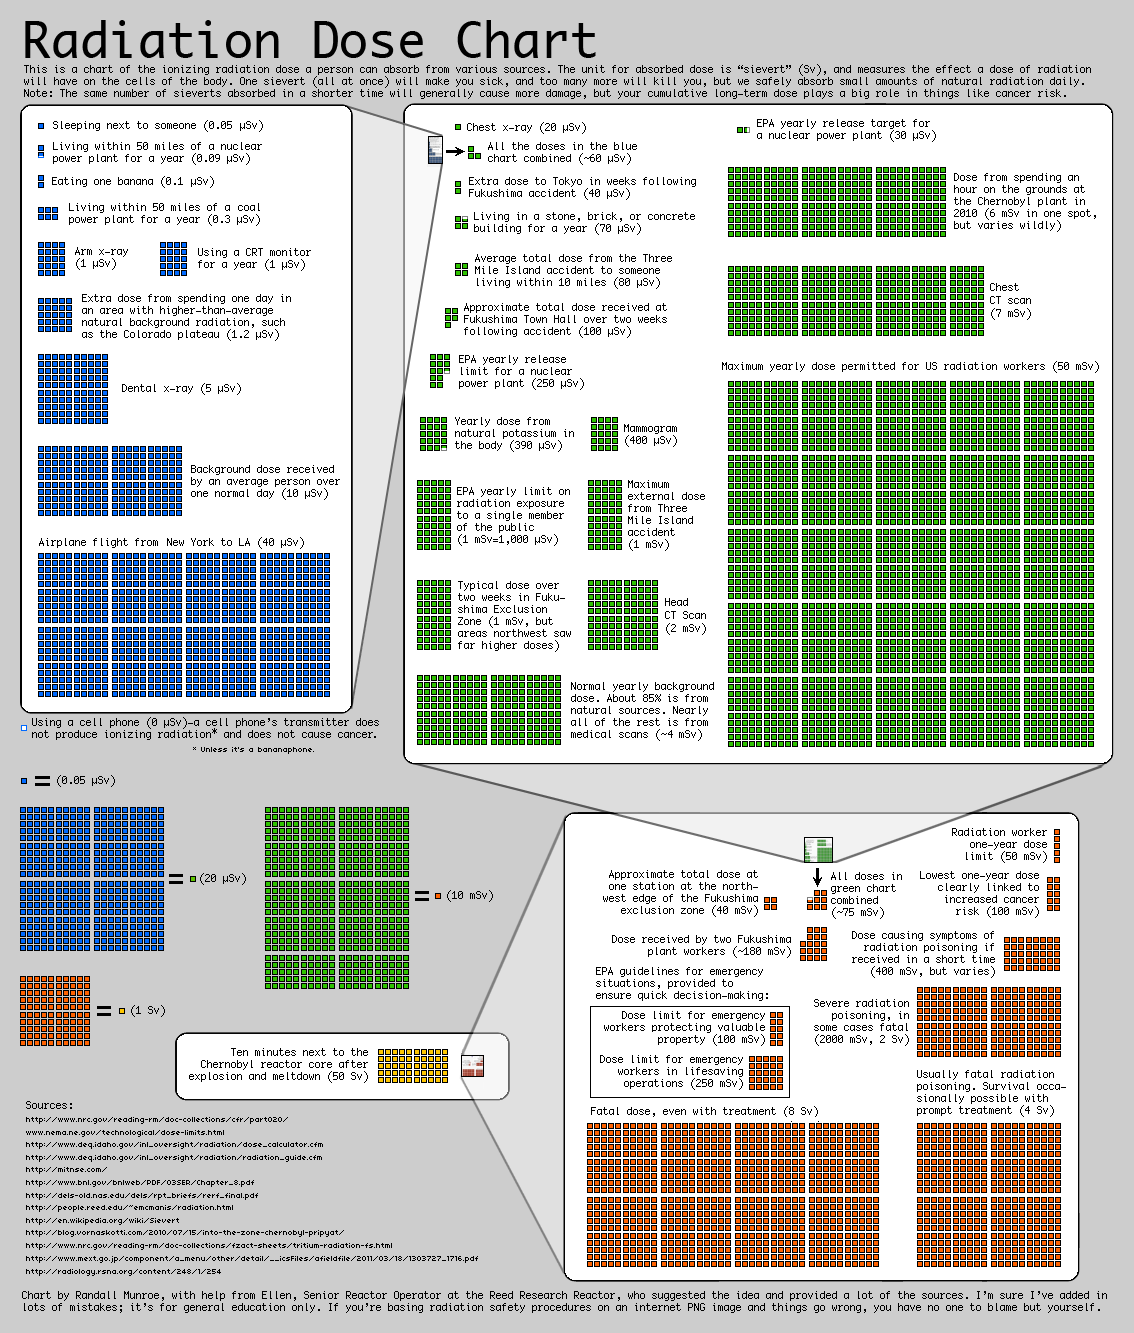
\includegraphics[width=\textwidth]{radioactivity-1/radiation-xkcd}
	\caption{A chart of ionizing radiation dose from various sources. Source: \url{https://xkcd.com/radiation/}}\label{rad1:doses}
\end{figure}

\textbf{Rubrics to focus on during this experiment:} C1, C4, C7, C8, F1, F2, G2. See Appendix~\ref{cha:rubrics} for details.

\subsection{Theory of counting statistics}

If you've ever worked in a not-too-busy retail environment, you’ve probably had the
experience of realizing (perhaps) that random and uniform are two quite different things.
You no doubt have sat waiting for customers, with nobody around for long stretches of
time, and then, as though they'd coordinated in advance, a half dozen people all show up
within a few minutes of each other. Each customer is indeed independent (no, they didn't
have a Twitter call to organize a flashmob!\footnote{Yes, popular interest in flash mobs peaked in 2011. Bear with us here.}) yet their arrival times clearly appear clustered. They are, in fact. But randomly. Uniform – one customer each minute – is quite dramatically different than a random procedure that yields one customer per minute on average. Retail customers (to a great extent), and elementary particles, act randomly, not uniformly.

Each atom in a radioactive sample has, per unit time, some probability of undergoing
radioactive decay. That probability is independent of all the other atoms in the sample.
Each atom decays, or not, based on its own probability and no other. The ensemble of
particle decay counts that one would measure in the sample (using a Geiger counter as we will
do, for example) is described by the something called the Poisson distribution, which
gives, in this instance, the probability of a integer number of events occurring in a fixed
interval of time, given an average rate. For large count rates, like we have here, the
Poisson distribution is indistinguishable from the normal distribution (that is, a simple
Gaussian function).

Specifically, for a process that produces an average $\bar{N}$ counts in a certain time duration (in the case of large $N$), the expected measurement of that count for that time duration is a
random draw from a normal distribution with mean $\bar{N}$ and a standard deviation of
$\sqrt{N}$.

\subsection{Doing the experiment}

\begin{enumerate}
	\item To find the steps of a testing experiment, review Rubric C, found in Table~\ref{rubric:c}.
	
	\item\label{rad1:step:predict-random} A prediction is what the hypothesis says will happen in the event of a particular experimental procedure. Given the hypothesis stated in the goal, and the theory described above, if you collect a series of counts of radioactive decay, what does the hypothesis predict the standard deviation of those counts should be equal to? Record this prediction in your lab notebook.
	
	\item \textbf{Collecting data.} In order to find the standard deviation of a number of measurements, you will need to take those measurements. In the following steps, you will do 10 trials of measuring the count rate (counts per unit time) during periods of about 30 seconds, then take the standard deviation of those 10 trials. Since you will not be able to stop the counter after exactly 30 seconds, you will divide the displayed count by the displayed time to get a count rate (in units of ``counts per second'').
	
	\begin{framed}
		\textbf{The Apparatus.}
		
		For this lab and the following one, you will be provided with a number of different radioactive materials packaged in small plastic disks. Note that each disk has the name of
		the isotope (e.g.\ $^{60}$Co), the type of radiation, and the half-life printed on one side of the
		sample. Half lives can range from fractions of a second to billions of years, depending on
		the isotope.
		
		The energetic particles produced in radioactive decay reactions can be detected by a
		device called a Geiger counter. This consists of a tube filled with inert gas with a wire
		running through it. A high voltage is applied between the wire and the tube. When a high-
		energy particle enters the tube, it can ionize the gas. The freed electrons produce a brief
		pulse of current at the output of the device. The pulses can then be counted.
		
		The counter itself is controlled using buttons on the front panel. \texttt{COUNT} begins the count
		and starts the timer, \texttt{STOP} pauses the count and timer, and \texttt{RESET} sets the count and
		timer to zero. Use the dial on the counter to change the display between the count and the
		elapsed time. When you first turn on the Geiger counter you need to set the voltage to
		$1000\:$V --- the TA will demonstrate how. \textbf{Caution:} Do not turn off the voltage during the
		experiment; use the \texttt{STOP} button to stop the count. \textbf{Do not touch the window on the
		bottom of the tube, as it breaks extremely easily.}
	\end{framed}
	\begin{enumerate}
		\item Take one of the $^{137}$Cs disks and place it printed side down in the plastic shelf shaped to hold it, and place that shelf in the slot second from the top in the stand under the Geiger counter. Note that if you have the Geiger counter on, that it is measuring a large count rate.
		
		\item Use the controls \texttt{COUNT}, \texttt{STOP}, and \texttt{RESET} to measure the number of counts in 10 approximately 30-second intervals. Use the dial on the display to access both the counts and the elapsed time. The provided stopwatch may also help you organize your effort --- \textit{but use the time from the Geiger counter apparatus directly} for your calculations.
		
		\item Record the counts and elapsed time in each interval in a spreadsheet and calculate the count rate in counts per minute (``cpm'' for short).
	\end{enumerate}

	\item \textbf{Analysis.} Note that the count rate is not identical in each trial, even though you accounted for the different measurement durations. Let's see how far away the standard deviation here is from the prediction in Step\ref{rad1:step:predict-random}. Calculate the standard deviation of these measurements. How close is it?
	
	\item Qualitatively, it might appear close or far away, but to test the hypothesis, you should take into account the uncertainty of the standard deviation. This is, effectively, the \textit{standard deviation of the standard deviation}. You would need to take, for example, 10 trials of these 10 trials and compute the standard deviation of that. Fortunately, you have other lab groups who are doing the same experiment. Share the standard deviation you found with the other lab groups, calculate the average and standard deviation of those standard deviations, and use Appendix~\ref{unc:sec:comparing} to compare your average standard deviation to the prediction that your hypothesis made.
	
	\item Use this quantitative comparison to determine if the prediction and the outcome agree or not.
	
	\item Based on that agreement, and taking into account the experimental conditions, make a judgment about the hypothesis.
\end{enumerate}
\chapter{Radioactive Half-Life}

%TODO add instructor note: to close door to KPTC 003, need to toggle switch that keeps it open, which is above the door.

%TODO add notes about neutron howitzer from https://wiki.uchicago.edu/display/phylabs/Mass+of+the+Neutron and from this email from David McCowan:
%The source is a mixture of plutonium and beryllium. The plutonium decays via alpha emission and the beryllium absorbs the alpha to become carbon + a free neutron. The neutron has an energy given by a very complicated distribution, but the energy distribution goes up to ~11 MeV. The paraffin shielding (and the lucite in the plug) slows down neutrons, so that anything which escapes is thermalized such that E ~ kT ~ 1/40 eV. At the point where the foils are placed, the neutrons have been slowed some, but not completely... if they are a full 11 MeV still, they are too energetic to bind with the silver, so the foils are absorbing from the lower end of the spectrum or from neutrons that have scattered enough material to have less energy than they started with.
%
%The activity of the Pu-Be core is an astounding 5 Ci (!!), but that's the alpha flux which doesn't penetrate out of the core. The neutron flux is considerably less. Looking back at the original purchase order, it looks like we have 80 g of plutoinium mixed with 41 g of beryllium and a listed (I think unshielded?) emission rate of 9 x 10^6 N/sec.

%TODO include suggestion to video the counter and a stopwatch to get more accurate 30-sec readings.

Building on our work from last week, we will continue to study the radioactive decay.
The physical laws of radioactivity predict that the rate of decay (number of atoms
decayed / time interval) is proportional to the number of radioactive nuclei present. This
is due, as we saw in counting statistics previously, to the independence of the decay of
each atom in the sample. The proportionality constant that describes the decay rate
depends on the specific radioactive nucleus. A concise and suggestive way to
characterize the nucleus is by its half-life, the time it takes for the number of radioactive
nuclei to decrease to half of the initial value. You will obtain data to check the form of
the law and to determine the half-life of one or more isotopes of silver.

We will use a device known as a neutron ``Howitzer''. It consists of a source of alpha
particles and a material that absorbs alpha particles and immediately decays by emitting
neutrons. (The neutrons shoot out from the barrel of the shielded volume, vaguely like
shells from WWI artillery, hence the name.)

\section{Background}

We will let the neutrons bombard a small sample of the stable isotope of silver, $^{107}$Ag, to
produce $^{108}$Ag, via the reaction
\begin{equation}
 ^{107}\textrm{Ag} + \mathrm{n} \rightarrow\, ^{108}\textrm{Ag} + \gamma \,,
\end{equation}
where $\mathrm{n}$ represents a neutron and $\gamma$ a gamma particle --- that is, a high energy photon.

The radioactive isotope of silver, $^{108}$Ag, spontaneously decays to an isotope of cadmium
with the same mass number, $^{108}$Cd, by the reaction
\begin{equation}
 ^{108}\textrm{Ag} \rightarrow\, ^{108}\textrm{Cd} + \mathrm{e}^- + \gamma \,,
\end{equation}
where $\mathrm{e}^-$ is an electron (that is, a $\beta$ particle, as we saw and measured last week).

Your TA will bombard silver foils with neutrons using the neutron howitzer. Some of the
nuclei in the foil will have captured a neutron and transformed into a different isotope
which is unstable and can be detected via their decay products. Each group will be given
one of these silver foils.

\section{Procedure}

\textbf{Rubric rows to be assessed:} D1, D4, F1, F2, G2, G3 (ignore actually doing it), G4

Your task is to measure the half-life of $^{108}$Ag. We will use the Geiger tube to count
decays. That is, we will count the $\beta$ particles --- the gamma rays make only a small
contribution to the counts in this instance. You should attempt to carry out the counting
fairly quickly after the silver foil is removed from the howitzer as the decay time is quite
short.

Before the neutron irradiation begins you will want to record the background rate. Press
\texttt{STOP} and \texttt{RESET} on the counter to set the display to zero. Next, press \texttt{COUNT} with no
sample below the Geiger tube and collect the total number of background counts, $N_\textrm{bkg}$ ,
that accumulate in approximately 5 minutes. Once 5 minutes has elapsed press \texttt{STOP} to
end the count. Turn the dial to \texttt{TIME} and record a precise measurement of the elapsed
time, $t$, in seconds. The background rate $R_\textrm{bkg}$ is found with
\begin{equation}
R_\textrm{bkg} = N_\textrm{bkg} /t
\end{equation}
with an uncertainty given by Poisson statistics. Report both the background rate and uncertainty in your lab report.

While the samples are being irradiated, set up your measurement apparatus. Once the samples are ready, quickly place a silver foil sample in the tray below the Geiger tube. Using a stopwatch and the
counter, record the number of counts and the time at 30 second intervals for
about 10 minutes, continuously. Unlike last week's lab with the same apparatus, you will
be recording data continuously, and so will need to use the watch to record times rather
than timer built into the Geiger counter. Record your data.

\section{Calculations}

The experimental data will be used to determine a half-life (or half-lives). We know that
the decay rate ($R=\Delta N / \Delta t$) of a radioactive nuclide is proportional to the number of nuclei present. The proportionality constant is called the decay constant $\lambda$, and the equation that describes what was just discussed is
\begin{equation}
 R = \lambda N \,,
\end{equation}
where $N$ is the background-subtracted counts. Using integral calculus and the above equation, we find
\begin{equation}
 N = N_0 e^{-\lambda t} \,,
\end{equation}
where $N_0$ is the number of nuclei at the initial time $t=0$. The half life $T_{1/2}$ is defined by
the time it takes for $N = N_0 /2$ and is related to the decay constant by $T_{1/2} = \ln(2)/ \lambda$, where
$\ln()$ is the natural logarithm function, and so $\ln(2) \approx 0.693$.

We can now write the radioactive decay equation as
\begin{equation}
 R = \lambda N_0 e^{-t \ln(2) / T_{1/2}} \,.
\end{equation}
Taking the logarithm of both sides and substituting for $N$ gives
\begin{equation}
 \ln(R) = - \left(\frac{\ln(2)}{T_{1/2}} \right) t + \mathrm{const} \,.
\end{equation}
Your TA will help you to understand the details of this derivation.

Make a plot showing $\ln(R)$ on the vertical axis and elapsed time, $t$, along the horizontal
axis. Don’t forget to subtract the background where appropriate. Calculate the slope
and use this value to solve for the half life using the above equations. Report this value
along with a table of your decay rate data and the plot described above.

\section{Questions (these should be included in your lab report)}

\begin{enumerate}
	\item Look up the half-lives of the various nuclides of silver. What is the published
	half-life of the nuclide you’re observing? How does this compare with your
	calculated result? Calculate the percent difference in your result.
	
	\item For the silver foil, how long would it take before you would expect to detect only
	one count per second, background corrected?
	
	\item The detector only measures particles that travel up into the detector. The majority
	of particles traveling in the other directions escape detection. Will this short-
	coming affect the measured half-life? If so, how? If not, why not?
	
	\item Describe one thing you could change in this experiment that could lead to a more
	accurate measurement of the half-life of the silver isotope.
	
	\item The particular irradiated silver sample you used contained some unknown
	percentage of the unstable silver isotope, and was irradiated at some unmeasured
	time before you began your experiment. Does this matter to your results? Explain.
	
\end{enumerate}

\appendix

\chapter{Analysis of Uncertainty}

A physical quantity consists of a value, unit, and uncertainty.
For example, ``$5 \pm 1\,$m'' means that the writer believes the true value of the quantity to most likely lie within 4 and 6 meters\footnote{The phrase ``most likely'' can mean different things depending on who is writing.
	If a physicist gives the value and does not given a further explanation, we can assume that they mean that the measurements are randomly distributed according to a normal distribution around the value given, with a standard deviation of the uncertainty given.
	So if one were to make the same measurement again, the author believes it has a 68\% chance of falling within the range given.
	Disciplines other than physics may intend the uncertainty to be 2 standard deviations.}.
Without knowing the uncertainty of a value, the quantity is next to useless.
For example, in our daily lives, we use an implied uncertainty.
If I say that we should meet at around 5:00 pm, and I arrive at 5:05 pm, you will probably consider that within the range that you would expect.
Perhaps your implied uncertainty is plus or minus 15 minutes.
On the other hand, if I said that we would meet at 5:07 pm, then if I arrive at 5:10 pm, you might be confused, since the implied uncertainty of that time value is more like 1 minute.

Scientists use the mathematics of probability and statistics, along with some intuition, to be precise and clear when talking about uncertainty, and it is vital to understand and report the uncertainty of quantitative results that we present.

\section{Types of measurement uncertainty}

For simplicity, we limit ourselves to the consideration of two types of uncertainty in this lab course, instrumental and random uncertainty.

\subsection{Instrumental uncertainties}

Every measuring instrument has an inherent uncertainty that is determined by the precision	
  of the instrument.
Usually this value is taken as a half of the smallest increment of the instrument's scale. For example, $0.5\:$mm is the precision of a standard metric ruler; $0.5\:$s is the precision of a watch, etc. For electronic digital displays, the equipment's manual often gives the instrument's resolution, which may be larger than that given by the rule above.

Instrumental uncertainties are the easiest ones to estimate, but they are not the only source of the uncertainty in your measured value.
You must be a skillful experimentalist to get rid of all other sources of uncertainty so that all that is left is instrumental uncertainty.

\subsection{Random uncertainties}

Very often when you measure the same physical quantity multiple times, you can get different results each time you measure it.
That happens because different uncontrollable factors affect your results randomly.
This type of uncertainty, random uncertainty, can be estimated only by repeating the same measurement several times.
For example if you measure the distance from a cannon to the place where the fired cannonball hits the ground, you could get different distances every time you repeat the same experiment.	
  
For example, say you took three measurements and obtained 55.7, 49.0, 52.5, 42.4, and 60.2 meters. We can quantify the variation in these measurements by finding their standard deviation using a calculator, spreadsheet, or the formula (assuming the data distributed according to a normal distribution)
\begin{equation}
 \sigma = \sqrt{\sum_{i=1}^{N} \frac{(x_i-\bar{x})^2}{N-1}} \, ,
\end{equation}
where $\{x_1, x_2, \dots, x_N\}$ are the measured values, $\bar{x}$ is the mean of those values, and $N$ is the number of measurements.
For our example, the resulting standard deviation is 6.8 meters. Generally we are interested not in the variation of the measurements themselves, but how uncertain we are of the average of the measurements. The uncertainty of this mean value is given, for a normal distribution, by the so-called ``standard deviation of the mean'', which can be found by dividing the standard deviation by the square root of the number of measurements,
\begin{equation}
\sigma_\textrm{mean} = \frac{\sigma}{\sqrt{N}} \, .
\end{equation}
So, in this example, the uncertainty of the mean is 3.0 meters. We can thus report the length as $52 \pm 3\:$m.

Note that if we take more measurements, the standard deviation of those measurements will not generally change, since the variability of our measurements shouldn't change over time. However, the standard deviation of the mean, and thus the uncertainty, will decrease.

\section{Propagation of uncertainty}

When we use an uncertain quantity in a calculation, the result is also uncertain. To determine by how much, we give some simple rules for basic calculations, and then a more general rule for use with any calculation which requires knowledge of calculus. Note that these rules are strictly valid only for values that are normally distributed, though for the purpose of this course, we will use these formulas regardless of the underlying distributions, unless otherwise stated, for simplicity.

If the measurements are completely independent of each other, then for quantities $a \pm \delta a$ and $b \pm \delta b$, we can use the following formulas:
\begin{equation}\label{unc:add}
\textrm{For } c = a + b \textrm{ (or for subtraction), } \delta c = \sqrt{(\delta a)^2 + (\delta b)^2}
\end{equation}

\begin{equation}\label{unc:mult}
\textrm{For } c = ab \textrm{ (or for division), } \frac{\delta c}{c} = \sqrt{\left(\frac{\delta a}{a}\right)^2 + \left(\frac{\delta b}{b}\right)^2}
\end{equation}

\begin{equation}\label{unc:exp}
\textrm{For } c = a^n,\, \frac{\delta c}{c} = n \frac{\delta a}{a}
\end{equation}

If you are familiar with calculus, you may want to use this general formula for the uncertainty $\delta f$ of a function $f$ of $N$ independent values $x_i$, each with uncertainty $\delta x_i$:
\begin{equation}\label{unc:general}
\delta f = \sqrt{ \sum_{i=1}^{N} \left(\frac{\partial f}{\partial x_i} \delta x_i\right)^2 } \, .
\end{equation}
Notice that Eqs.\ \ref{unc:add} through \ref{unc:exp} can be derived from Eq.\ \ref{unc:general} for those specific cases.

\subsubsection{What if there is no reported uncertainty?}

Sometimes you'll be calculating with numbers that have no uncertainty given.
In some cases, the number is exact.
For example, the circumference $C$ of a circle is given by $C = 2 \pi r$. Here, the coefficient, $2\pi$, is an exact quantity and you can treat its uncertainty as zero.
If you find a value that you think is uncertain, but the uncertainty is not given, a good rule of thumb is to assume that the uncertainty is half the right-most significant digit.
So if you are given a measured length of $1400\:$m, then you might assume that the uncertainty is $50\:$m.
This is an assumption, however, and should be described as such in your lab report.
For more examples, see Table~\ref{unc:tab:implied}.

\begin{table}
	\begin{center}
		\begin{tabular}{cc}
			\textbf{Expression} & \textbf{Implied uncertainty} \\
			12 & 0.5 \\
			12.0 & 0.05 \\
			120 & 5 \\
			120. & 0.5
		\end{tabular}
		\caption{Expression of numbers and their implied uncertainty.}\label{unc:tab:implied}
	\end{center}
\end{table}

\subsubsection{How many digits to report?}

After even a single calculation, a calculator will often give ten or more digits in an answer.
For example, if I travel $11.3 \pm 0.1\:$km in $350 \pm 10\:$s, then my average speed will be the distance divided by the duration. Entering this into my calculator, I get the resulting value ``\texttt{0.0322857142857143}''.
Perhaps it is obvious that my distance and duration measurements were not precise enough for all of those digits to be useful information.
We can use the propagated uncertainty to decide how many decimals to include.
Using the formulas above, I find that the uncertainty in the speed is given by my calculator as ``\texttt{9.65683578099600e-04}'', where the `\texttt{e}' stands for ``times ten to the''.
I definitely do not know my uncertainty to 14 decimal places.
For reporting uncertainties, it general suffices to use just the 1 or 2 left-most significant digits, unless you have a more sophisticated method of quantifying your uncertainties.
So here, I would round this to 1 significant digit, resulting in an uncertainty of $0.001\:$km/s.
Now I have a guide for how many digits to report in my value.
Any decimal places to the right of the one given in the uncertainty are distinctly unhelpful, so I report my average speed as ``$0.032 \pm 0.001\:$km/s''.
You may also see the equivalent, more succinct notation ``$0.032(1)\:$km/s''.

\section{Comparing two values}\label{unc:sec:comparing}

If we compare two quantities and want to find out how different they are from each other, we can use a measure we call a $t'$ value (pronounced ``tee prime''). This measure is not a standard statistical measure, but it is simple and its meaning is clear for us.

Operationally, for two quantities having the same unit, $a \pm \delta a$ and $b \pm \delta b$, the measure is defined as\footnote{Statistically, if $\delta a$ and $\delta b$ are uncorrelated, random uncertainties, then $t'$ represents how many standard deviations the difference $a - b$ is away from zero.}

\begin{equation}
%t' = \frac{\abs{a-b}}{\sqrt{(\delta a)^2 + (\delta b)^2}}
t' = \frac{\abs{a-b}}{\sqrt{(\delta a)^2 + (\delta b)^2}}
\end{equation}

If $t' \lesssim 1$, then the values are so close to each other that they are indistinguishable. It is either that they represent the same true value, or that the measurement should be improved to reduce the uncertainty.

If $1 \lesssim t' \lesssim 3$, then the result is inconclusive. One should improve the experiment to reduce the uncertainty.

If $t' \gtrsim 3$, then the true values are very probably different from each other.
\begin{landscape}
\chapter{Rubrics}
	
	\freetabcaption{Rubric B: Ability to design and conduct an observational experiment \cite{etkina_scientific_2006}.}
	\begin{longtable}{>{\bfseries}p{0.02\textheight}|>{\bfseries\RaggedRight}p{0.25\textheight}|>{\RaggedRight}p{0.21\textheight}|>{\RaggedRight}p{0.21\textheight}|>{\RaggedRight}p{0.22\textheight}|>{\RaggedRight}p{0.22\textheight}}
		\toprule
		& Scientific Ability
		& Missing & Inadequate & Needs Improvement & Adequate \\ \midrule \endhead
		B1
		& Is able to identify the phenomenon to be investigated
		& No phenomenon is mentioned
		& The description of the phenomenon to be investigated is confusing, or it is not the phenomenon of interest.
		& \midsloppy The description of the phenomenon is vague or incomplete.
		& The phenomenon to be investigated is clearly stated. \\ \midrule
		B2
		& Is able to design a reliable experiment that investigates the phenomenon
		& The experiment does not investigate the phenomenon.
		& The experiment may not yield any interesting patterns.
		& Some important aspects of the phenomenon will not be observable.
		& The experiment might yield interesting patterns relevant to the investigation of the phenomenon. \\ \midrule
		B3
		& Is able to decide what physical quantities are to be measured and identify independent and dependent variables
		& The physical quantities are irrelevant.
		& Only some of physical quantities are relevant.
		& The physical quantities are relevant. However, independent and dependent variables are not identified.
		& The physical quantities are relevant and independent and dependent variables are identified. \\ \midrule
		B4
		& Is able to describe how to use available equipment to make measurements
		& At least one of the chosen measurements cannot be made with the available equipment.
		& All chosen measurements can be made, but no details are given about how it is done.
		& All chosen measurements can be made, but the details of how it is done are vague or incomplete.
		& All chosen measurements can be made and all details of how it is done are clearly provided. \\ \midrule
		B5
		& Is able to describe what is observed without trying to explain, both in words and by means of a picture of the experimental setup.
		& No description is mentioned.
		& A description is incomplete. No labeled sketch is present. Or, observations are adjusted to fit expectations.
		& A description is complete, but mixed up with explanations or pattern. Or the sketch is present but is difficult to understand.
		& Clearly describes what happens in the experiments both verbally and with a sketch. Provides other representations when necessary (tables and graphs). \\ \midrule
		B6
		& Is able to identify the shortcomings in an experiment and suggest improvements
		& No attempt is made to identify any shortcomings of the experiment.
		& The shortcomings are described vaguely and no suggestions for improvement are made.
		& Not all aspects of the design are considered in terms of shortcomings or improvements.
		& All major shortcomings of the experiment are identified and reasonable suggestions for improvement are made. \\ \midrule
		B7
		& Is able to identify a pattern in the data
		& No attempt is made to search for a pattern.
		& The pattern described is irrelevant or inconsistent with the data.
		& The pattern has minor errors or omissions. Terms like ``proportional'' used without clarity, e.g.\ is the proportionality linear, quadratic, etc.
		& The pattern represents the relevant trend in the data. When possible, the trend is described in words. \\ \midrule
		B8
		& Is able to represent a pattern mathematically (if applicable)
		& No attempt is made to represent a pattern mathematically.
		& The mathematical expression does not represent the trend.
		& No analysis of how well the expression agrees with the data is included, or some features of the pattern are missing.
		& The expression represents the trend completely and an analysis of how well it agrees with the data is included. \\ \midrule
		B9
		& Is able to devise an explanation for an observed pattern
		& No attempt is made to explain the observed pattern.
		& An explanation is vague, not testable, or contradicts the pattern.
		& An explanation contradicts previous knowledge or the reasoning is flawed.
		& A reasonable explanation is made. It is testable and it explains the observed pattern. \\
		\bottomrule
	\end{longtable}

	
%\end{table}

\end{landscape}
\chapter{Lab Report Format}

Following the last session of a particular lab, each person will be responsible for turning in a lab report. In a general sense, the labs should demonstrate Rubric Rows F1 and F2 (see Table~\ref{rubric:f}), in addition to the other rubric rows listed in the lab write-up.

\section{General}

\begin{itemize}
	\item The report should be typed for ease of reading. Text should be double-spaced, and the page margins (including headers and footers) should be approximately $2.5\:$cm, for ease of marking by the grader. Each page should be numbered.
	
	\item The first page should include the title of the lab; lab section day, time, and number; and the names of the other members of your lab team.
	
	\item If the rubric row refers to a particular part of your lab report, clearly label that part of the report with that rubric row. For example, you should label the section where you demonstrate uncertainty propagation with ``G2'' if that rubric row is being assessed in that lab.
\end{itemize}

\section{Organizing the report}

If the lab is clearly framed as an observational, testing, or application experiment, you can follow the corresponding rubric for the elements to include in the report (see, respectively, Rubrics B, C, and D in Appendix~\ref{cha:rubrics}).

In general, the report \textbf{must} include the following sections:
\begin{enumerate}
	\item \textbf{Introduction.} A written description of what the lab is designed to investigate and a brief summary of the procedure used. This section should be at least a full paragraph long, and not more than 3 double-space pages.
	
	You don't need to include too much detail here, but it should be a complete and concise description of the purpose and general method used in the lab. Imagine a classmate who hasn't seen the lab writeup asked you, ``what is this lab about? What do you do?'' You should be able to hand them your introduction, and they'd be able to understand the purpose and general structure of the lab. But you need not mention every step and calculation here.
	
	\item \textbf{Analysis and discussion.} For most labs that have more than one part, this should be broken up into parts and labeled in order. This section must include all of the following, in the same order in which these elements appear in the lab instructions.
	\begin{itemize}
		\item Any data that you've collected: tables, figures, measured values, sketches. Whenever possible, include an estimate of the uncertainty of measured values.
		
		\item Any calculations that you perform using your data, and the final results of your calculation. Note that you must show your work in order to demonstrate to the grader that you have actually done it. Even if you're just plugging numbers into an equation, you should write down the equation and all the values that go into it. This includes calculating uncertainty and propagation of uncertainty.
		
		\item If you are using software to perform a calculation, you should explicitly record what you've done. For example, ``Using Excel we fit a straight line to the velocity vs. time graph. The resulting equation is $v = (0.92\:\mathrm{m/s^2}) t + 0.2\:\mathrm{m/s}$.
		
		\item Answers to any questions that appear in the lab handout.
	\end{itemize}

	\item \textbf{Conclusion.} This can be very short, and will generally only require one or two paragraphs. In your conclusion, you should summarize the point of the lab and what you learned, both in the frame of a scientist conducting the experiment (``What did the experiment tell us about the world?'') and in the frame of a student (``What skills or mindsets did I learn?'').
\end{enumerate}

\section{Graphs, Tables, and Figures}

Any graph, table, or figure (a figure is any graphic, for example a sketch) should include a caption describing what it is about and what features are important, or any helpful orientation to it. The reader should be able to understand the basics of what a graph, table, or figure is saying and why it is important without referring to the text. For more examples, see any such element in this lab manual.

Each of these elements has some particular conventions.

\subsection{Tables}

A table is a way to represent tabular data in a quantitative, precise form. Each column in the table should have a heading that describes the quantity name and the unit abbreviation in parentheses. For example, if you are reporting distance in parsecs, then the column heading should be something like ``distance (pc)''. This way, when reporting the distance itself in the column, you do not need to list the unit with every number.

\subsection{Graphs}

A graph is a visual way of representing data. It is helpful for communicating a visual summary of the data and any patterns that are found.

The following are necessary elements of a graph of two-dimensional data (for example, distance vs. time, or current vs. voltage) presented in a scatter plot.

\begin{itemize}
	\item \textbf{Proper axes.} The conventional way of reading a graph is to see how the variable on the vertical axis changes when the variable on the horizontal axis changes. If there are independent and dependent variables, then the independent variable should be along the horizontal axis.
	
	\item \textbf{Axis labels.} The axes should each be labeled with the quantity name and the unit abbreviation in parentheses. For example, if you are plotting distance in parsecs, then the axis label should be something like ``distance (pc)''.
	
	\item \textbf{Uncertainty bars.} If any quantities have an uncertainty, then these should be represented with so-called ``error bars'', along both axes if present. If the uncertainties are smaller than the symbol used for the data points, then this should be explained in the caption.

\end{itemize}


% \bibliography{references,MyLibrary}
% \bibliographystyle{plain}
\printbibliography

\end{document}
